\icode{E-MCC-MU-L3-261024-001}
自动计数的智能呼啦圈其模型如图所示，水平固定的圆形腰带外侧有轨道，配重通过轻绳与轨道上的滑轮\(P\)连接。	锻炼中，配重的运动简化为绕腰带的中心轴在水平面内匀速转动。已知配重的质量为\(m\)，轻绳长为\(l\)，与竖直方向的夹角为\(\theta\)，圆形腰带的半径为\(r\)，重力加速度为\(g\)，配重可视为质点，则配重\paren[]

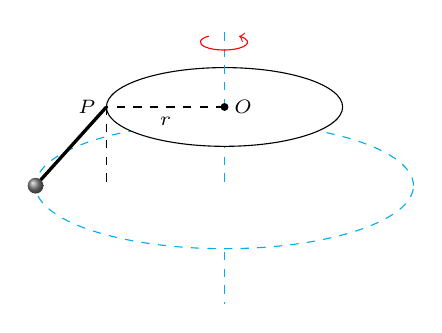
\begin{tikzpicture}[font=\scriptsize]
	\draw[dashed,cyan] (0,-1)--(0,-2.5);
	\draw[dashed,cyan,fill=white] (0,-1) ellipse(2.4 and .8);
	\draw[dashed,cyan] (0,0)--(0,-1);
	\draw[fill=white] (0,0) ellipse(1.5 and .5);
	\draw[dashed,cyan] (0,0)--(0,1);
	\fill (0,0)node[right]{\(O\)} circle(.05);
	\draw[very thick] (-1.5,0)node[left]{\(P\)}--(-2.4,-1);
	\shade[ball color=gray] (-2.4,-1) circle(.1);
	\draw[dashed] (-1.5,0)--(-1.5,-1) (0,0)--node[below]{\(r\)}(-1.5,0);
	\draw[->,red] (-.2,.9) arc (-230:50:.3 and .1);
\end{tikzpicture}
\begin{choices}
	\item 受到的拉力大小为\(T = mg\sin\theta\)
	\item 受到的拉力大小为\(T = \dfrac{mg}{\cos\theta}\)
	\item 转动的角速度为\(\omega = \sqrt{\dfrac{g}{l\cos\theta}}\)
	\item 转动的角速度为\(\omega = \sqrt{\dfrac{g\tan\theta}{l\sin\theta + r}}\)
\end{choices}
\begin{answer}
    
\end{answer}
